\chapter{Kerr-Schild metrics}
\label{s:ksm}

\minitoc

\section{Generic Kerr-Schild spacetimes}

\subsection{Definition} \label{s:ksm:def_Kerr_Schild}

A spacetime $(\M,\w{g})$ is said to have a
\defin{Kerr-Schild metric}\index{Kerr-Schild!metric} iff the metric tensor $\w{g}$
can be written
\be \label{e:ksm:g_KerrSchild}
   \encadre{ \w{g} = \w{f} + 2 H \uu{k}\otimes\uu{k} },
\ee
or equivalently (in index notation):
\be \label{e:ksm:g_KerrSchild_comp}
    \encadre{ g_{\alpha\beta} = f_{\alpha\beta} + 2 H k_\alpha k_\beta },
\ee
where $\w{f}$ is a \emph{flat} Lorentzian metric on $\M$ (Minkowski metric\index{Minkowski!metric}),
$H$ is a scalar field on $\M$ and $\uu{k}$ is a 1-form on $\M$ such that the
vector associated to it via $\w{f}$ is a null vector of the metric
$\w{f}$:
\be
     f^{\mu\nu} k_\mu k_\nu = 0 ,
\ee
where $f^{\mu\nu}$ stands for the components of the inverse of the metric
$\w{f}$ (i.e. $f^{\alpha\mu} f_{\mu\beta} = \delta^\alpha_{\ \; \beta}$).

A motivation for studying
Kerr-Schild metrics is that the inverse metric has a simple expression:
\be \label{e:ksm:g_inverse}
    g^{\alpha\beta} = f^{\alpha\beta} - 2 H k^\alpha k^\beta ,
\ee
where
\be \label{e:ksm:k_up_comp}
    k^\alpha := f^{\alpha\mu} k_\mu .
\ee
\emph{Proof:} we have successively:
\bea
   (f^{\alpha\mu} - 2 H k^\alpha k^\mu) g_{\mu\beta} & = &
   (f^{\alpha\mu} - 2 H k^\alpha k^\mu) (f_{\mu\beta} + 2 H k_\mu k_\beta) \nonumber \\
   & = & \underbrace{f^{\alpha\mu} f_{\mu\beta}}_{\delta^\alpha_{\ \; \beta}}
    + 2 H \underbrace{f^{\alpha\mu} k_\mu}_{k^\alpha} k_\beta
    - 2 H k^\alpha \underbrace{k^\mu f_{\mu\beta}}_{k_\beta}
    - 4 H^2 k^\alpha \underbrace{k^\mu k_\mu}_{0} k_\beta \nonumber \\
   & = & \delta^\alpha_{\ \; \beta} , \nonumber
\eea
which establishes Eq.~\eqref{e:ksm:g_inverse}. \qed

Given (\ref{e:ksm:g_inverse}), it is easy to see that the vector field
$\w{k}$ associated
to the 1-form $\uu{k}$ by $\w{g}$-duality (cf. Sec.~\ref{s:bas:metric_dual})
is the same as the vector field
obtained by $\w{f}$-duality:
\[
    g^{\alpha\mu} k_\mu = (f^{\alpha\mu} - 2 H k^\alpha k^\mu) k_\mu
                        = \underbrace{f^{\alpha\mu} k_\mu}_{k^\alpha}
                          - 2H k^\alpha \underbrace{k^\mu k_\mu}_{0}
                        = k^\alpha .
\]
Accordingly, we may write the components of $\w{k}$ simply as $k^\alpha$
without having to specify whether the index has been raised with $\w{g}$ or $\w{f}$:
\be
    k^\alpha = f^{\alpha\mu} k_\mu  = g^{\alpha\mu} k_\mu .
\ee
It follows immediately that $\w{k}$ is a null vector field for
both metrics:
\be
   \encadre{ \w{g}(\w{k}, \w{k}) = \w{f}(\w{k}, \w{k}) = 0 }.
\ee


If $(\M,\w{g})$ is a spacetime of Kerr-Schild type, then \defin{Kerr-Schild
coordinates}\index{Kerr-Schild!coordinates}
are coordinates $(x^\alpha) = (t,x,y,z)$ that are \emph{Minkowskian}\index{Minkowskian coordinates}
for $\w{f}$, i.e. coordinates in which the flat metric
$\w{f}$ takes the form
\be \label{e:ksm:ds_eta}
    \w{f} = - \dd t^2 + \dd x^2 + \dd y^2 + \dd z^2 .
\ee

\subsection{Basic property}

\begin{prop}[null vector of Kerr-Schild metric as a geodesic vector]
Let $\w{g}$ be a Kerr-Schild metric.
If $\w{g}$ obeys the vacuum Einstein
equation\index{Einstein!equation!vacuum --}\index{vacuum!Einstein equation}
(\ref{e:fra:vac_Einstein}),
i.e. if the Ricci tensor of $\w{g}$ vanishes identically,
then the scalar field $H$ appearing in Eq.~(\ref{e:ksm:g_KerrSchild})
can be chosen so that $\w{k}$ is a geodesic vector field\footnote{See Sec.~\ref{s:geo:gener_param} for the definition of a geodesic vector field.}:
\be \label{e:ksm:k_geodesic}
    \encadre{ k^\mu \nabla_\mu k^\alpha = 0 },
\ee
where $\nabla$ stands for the covariant derivative associated with $\w{g}$.
\end{prop}

The proof of the above proposition can be found in Ref.~\cite{KerrS65}.


%%%%%%%%%%%%%%%%%%%%%%%%%%%%%%%%%%%%%%%%%%%%%%%%%%%%%%%%%%%%%%%%%%%%%%%%%%%%%%%

\section{Case of Kerr spacetime}

\subsection{Kerr-Schild form}

Let consider the Kerr spacetime $(\M,\w{g})$, where $\M$ is the manifold
(\ref{e:ker:def_M_Kerr_spacetime}): $\M = \R^2\times\SS^2 \setminus \ring$
and $\w{g}$ is the metric tensor given by Eq.~(\ref{e:ker:metric_Kerr_3p1})
in terms of the Kerr coordinates $(\ti, r, \th,\tph)$ introduced in
Sec.~\ref{s:ker:3p1_Kerr_coord}.
Let us show that $\w{g}$ is a Kerr-Schild metric, with the associated null vector
field $\w{k}$ being nothing but the vector field generating the
ingoing principal null geodesics\index{principal!null geodesic} $\Li^{\rm in}_{(v,\th,\tph)}$  discussed in Sec.~\ref{s:ker:principal_geod}.
Its expression in terms of the Kerr coordinates is given by Eq.~(\ref{e:ker:k_ti_tr}):
\be \label{e:ksm:k_Kerr}
    \encadre{ \w{k} = \wpar_\ti - \wpar_{\tilde r} } .
\ee
In other words, the components of $\w{k}$ with respect to the Kerr coordinates $(\ti, r, \th,\tph)$ are $k^\alpha = (1, -1, 0, 0)$.
The 1-form $\uu{k}$ associated to $\w{k}$ by $\w{g}$-duality is
given by Eq.~(\ref{e:ker:k_form_Kerr}):
\be \label{e:ksm:k_form_Kerr}
    \uu{k} = - \dd \ti - \dd r + a\sin^2\th \, \dd\tph .
\ee
Equivalently, $k_\alpha = (-1, -1, 0, a\sin^2\th)$.
Let us then introduce the symmetric bilinear form
\be
    \w{f} := \w{g} - 2 H \uu{k} \otimes \uu{k} ,
\ee
where $H$ is the following scalar field on $\M$:
\be \label{e:ksm:H_Kerr}
   \encadre{ H := \frac{m r}{\rho^2} },
\ee
with $\rho^2 := r^2 + a^2 \cos^2\th$ [Eq.~(\ref{e:ker:def_rho2})].
The expression of $\w{f}$ in terms of Kerr coordinates is deduced
from that of $\w{g}$ [Eq.~(\ref{e:ker:metric_Kerr_3p1})] and that of
$\uu{k}$ [Eq.~(\ref{e:ksm:k_form_Kerr})]:
\be \label{e:ksm:f_Kerr}
  \encadre{  \w{f} = - \dd\ti^2 + \dd r^2 - 2 a \sin^2\th \, \dd r \, \dd\tph
    + \rho^2\, \dd \th^2 + (r^2 + a^2)\sin^2\th\, \dd \tph^2 }.
\ee
It is easy to check that $f^{\alpha\beta} := g^{\alpha\beta} + 2 H k^\alpha k^\beta$
defines an inverse of $\w{f}$: $f^{\alpha\mu} f_{\mu\beta} = \delta^\alpha_{\ \; \beta}$
(computation similar to that in Sec.~\ref{s:ksm:def_Kerr_Schild}). Hence the
symmetric bilinear form $\w{f}$ is non-degenerate; this implies that $\w{f}$
is a \emph{metric tensor} on $\M$ (cf. Sec.~\ref{s:bas:metric}).
Given the components (\ref{e:ksm:k_form_Kerr}), it is immediate to check that $\w{k}$ is a null vector for $\w{f}$ as well: $\w{f}(\w{k}, \w{k}) = 0$.
Moreover, $\w{f}$ is a \emph{flat} metric, since a direct computation of its
Riemann tensor (cf. the notebook \ref{s:sam:Kerr_Schild}) reveals that
\be
    \mathrm{\bf Riem}(\w{f}) = 0 .
\ee
In view of the definition given in Sec.~\ref{s:ksm:def_Kerr_Schild},
we conclude:
\begin{prop}[Kerr metric as a Kerr-Schild metric]
The Kerr metric $\w{g}$ is a Kerr-Schild metric, i.e. it can be written in
the form (\ref{e:ksm:g_KerrSchild}) with the flat metric
$\w{f}$ given by Eq.~(\ref{e:ksm:f_Kerr}), the scalar field $H$ given
by Eq.~(\ref{e:ksm:H_Kerr}) and the null vector $\w{k}$ given by
Eq.~(\ref{e:ksm:k_Kerr}), $\w{k}$ being the tangent vector field to
the ingoing principal null geodesics.
\end{prop}
In Sec.~\ref{s:ker:principal_geod},
we have already noticed that $\w{k}$ is a geodesic vector:
$\wnab_{\w{k}}\, \w{k} = 0$ [Eq.~(\ref{e:ker:nab_k_k})], in agreement with
(\ref{e:ksm:k_geodesic}).

\begin{remark}
The Kerr metric can also be brought to the Kerr-Schild form by using the
tangent vector field to the  \emph{outgoing} principal null geodesics. Hence
the Kerr-Schild decomposition (\ref{e:ksm:g_KerrSchild}) is not unique for
the Kerr metric.
\end{remark}

\subsection{Kerr-Schild coordinates on Kerr spacetime}

It is not immediately obvious that the metric $\w{f}$ given by
Eq.~(\ref{e:ksm:f_Kerr}) is a flat Lorentzian metric, except at the limit $a=0$.
Let us introduce coordinates in which $\w{f}$ takes a manifest Minkowskian
form, i.e. Kerr-Schild coordinates, according to the nomenclature introduced
in Sec.~\ref{s:ksm:def_Kerr_Schild}.

Actually, if $a\not=0$, one cannot introduce a Kerr-Schild coordinate system on the whole
spacetime manifold $\M = \R^2\times\SS^2 \setminus \ring$ as defined by
Eq.~(\ref{e:ker:def_M_Kerr_spacetime}). One has to split it in two parts:
\begin{subequations}
\begin{align}
    \M & :=  \M_+ \cup \M_- , \\
    \M_+ & :=  \R\times {[0,+\infty)}\times\SS^2 \setminus \ring\\
    \M_- & :=  \R\times {(-\infty,0]}\times\SS^2 \setminus \ring .
\end{align}
\end{subequations}
In other words, $\M_+$ is the part $r\geq 0$ of $\M$, while $\M_-$ is the part
$r\leq 0$. Note that $\M_+$ and $\M_-$ are submanifolds with boundaries
(cf. Sec.~\ref{s:bas:manif_boundary}), which overlap at $r=0$. In terms of the domains introduced in Sec.~\ref{s:ker:expr_BL},
$\M_+$ contains $\M_{\rm I}$, $\M_{\rm II}$ and a part of $\M_{\rm III}$,
while $\M_-$ is entirely included in $\M_{\rm III}$.
The \defin{Kerr-Schild coordinates} $(\ti, x, y, z)$
on $\M_+$ are defined from the Kerr coordinates
$(\ti, r, \th,\tph)$ by the following formulas:
\begin{subequations}
\label{e:ksm:K_to_KS}
\bea
    \ti & = & \ti \\
    x & = & (r\cos\tph - a \sin\tph) \sin \th  \label{e:ksm:x_Kerr}\\
    y & = & (r\sin\tph + a \cos\tph) \sin \th  \label{e:ksm:y_Kerr}\\
    z & = & r\cos \th . \label{e:ksm:z_Kerr}
\eea
\end{subequations}

\begin{remark}
As we shall see in Sec.~\ref{s:ksm:r_zero}, the Kerr-Schild coordinates
are singular at $r=0$, so strictly speaking, we should have omitted $r=0$ from
the definition of $\M_+$ and $\M_-$.
\end{remark}

\begin{remark}
For $a=0$, Eqs.~\eqref{e:ksm:x_Kerr}-\eqref{e:ksm:z_Kerr} reduce to the standard
relations between Cartesian and spherical coordinates in Euclidean space.
\end{remark}
\begin{remark}
Equations~(\ref{e:ksm:x_Kerr})-(\ref{e:ksm:y_Kerr}) can be combined into a single
relation:
\be
    x + i y = (r + i a) \mathrm{e}^{i\tph} \sin\th .
\ee
\end{remark}
From Eqs.~(\ref{e:ksm:x_Kerr})-(\ref{e:ksm:y_Kerr}), we
get
\be
    x^2 + y^2 = (r^2 + a^2)\sin^2\th .
\ee
Combining with Eq.~(\ref{e:ksm:z_Kerr}) yields:
\be \label{e:ksm:ellipsoids}
\encadre{ \frac{x^2 + y^2}{r^2 + a^2} + \frac{z^2}{r^2} = 1 } .
\ee
This is a quadratic equation in $r^2$. Solving it results in
\be \label{e:ksm:r_xyz}
    r = \sqrt{ \frac{1}{2} \left(
        x^2 + y^2 + z^2 - a^2 +
        \sqrt{(x^2 + y^2 + z^2 - a^2)^2 + 4 a^2 z^2} \right)}  .
\ee

The components of $\w{f}$ in terms on the coordinates
$(x^\alpha)=(\ti, x, y, z)$ are obtained
via the tensor change-of-components formula with
the transformation (\ref{e:ksm:K_to_KS})
(cf. the notebook \ref{s:sam:Kerr_Schild}):
\be \label{e:ksm:f_Kerr_KS}
 \w{f} = - \dd\ti^2 + \dd x^2 + \dd y^2 + \dd z^2 .
\ee
This proves that $(\ti, x, y, z)$ are Kerr-Schild coordinates, as announced.

The expression of the vector $\w{k}$ in terms of the Kerr-Schild coordinates
is obtained similarly:
\be
    \w{k} = \wpar_{\ti} - \frac{r x + a y}{r^2 + a^2} \, \wpar_x
        - \frac{r y - a x}{r^2 + a^2} \, \wpar_y
        - \frac{z}{r}\, \wpar_z .
\ee
In this formula, $r$ is to be considered as the function of $(x,y,z)$ given
by Eq.~(\ref{e:ksm:r_xyz}). For the associated 1-form, we get
\be \label{e:ksm:k_form_Kerr_KS}
    \uu{k} = - \dd\ti - \frac{r x + a y}{r^2 + a^2} \, \dd x
       - \frac{r y - a x}{r^2 + a^2} \, \dd y
        - \frac{z}{r}\, \dd z .
\ee
The scalar factor $H$ can be re-expressed from Eq.~(\ref{e:ksm:H_Kerr})
in terms of $z$ and $r$:
\be \label{e:ksm:H_Kerr_zr}
    H = \frac{m r^3}{r^4 + a^2 z^2}  .
\ee

\begin{remark}
If $a=0$ (Schwarzschild limit), we get
\be \label{e:ksm:lim_a_zero}
    r = \sqrt{x^2 + y^2 + z^2}, \quad
    H = \frac{m}{r} \quad\mbox{and}\quad
    \uu{k} = - \dd\ti - \frac{x}{r} \, \dd x
       - \frac{y}{r} \, \dd y
        - \frac{z}{r}\, \dd z .
\ee
\end{remark}

\begin{remark}
For $a \not = 0$, the relations (\ref{e:ksm:lim_a_zero}) hold at first order
in the limit $r \gg a$, or equivalently in the limit $\sqrt{x^2 + y^2 + z^2} \gg a$.
\end{remark}

The explicit form of the components
$(g_{\alpha\beta})$ of the Kerr metric in Kerr-Schild coordinates can be read off by expanding
the following expression of $\w{g}$:
\be \label{e:ksm:g_comp_KS}
\encadre{ \begin{array}{ll}
 \w{g} = & - \dd \ti^2 + \dd x^2 + \dd y^2
        + \dd z^2 \\
        &\displaystyle  + \frac{2m r^3}{r^4 + a^2 z^2} \left( \dd \ti
        + \frac{r x + a y}{r^2 + a^2} \, \dd x
        + \frac{r y - a x}{r^2 + a^2} \, \dd y + \frac{z}{r} \, \dd z \right) ^2
\end{array} } ,
\ee
which is obtained by combining Eqs~(\ref{e:ksm:g_KerrSchild_comp}), (\ref{e:ksm:f_Kerr_KS}),
(\ref{e:ksm:H_Kerr_zr})
and (\ref{e:ksm:k_form_Kerr_KS}).
\begin{remark}
It is clear on \eqref{e:ksm:g_comp_KS} that all metric components in Kerr-Schild
coordinates are regular both at the the black hole event horizon
($r= m + \sqrt{m^2 - a^2}$, cf. Sec.~\ref{s:ker:event_hor}) and the Cauchy horizon
($r = m - \sqrt{m^2 - a^2}$, cf. Sec.~\ref{s:ker:Cauchy_hor}).
This property, which is shared by the Kerr coordinates,
is in sharp contrast with the metric components in
Boyer-Lindquist coordinates, which are singular at both horizons (cf. Sec.~\ref{s:ker:singularities}).
\end{remark}

Finally, the axisymmetry Killing vector $\w{\eta} = \wpar_\tph$
of Kerr spacetime [Eq.~(\ref{e:ker:Killing_vec_3p1})] has the following
expression in terms of Kerr-Schild coordinates:
\be \label{e:ksm:eta_KS}
    \w{\eta} = - y\, \wpar_x + x \, \wpar_y .
\ee
This is easily established from the chain rule and the partial
derivative with respect to $\tph$ of expressions (\ref{e:ksm:K_to_KS}).
We notice on Eq.~(\ref{e:ksm:eta_KS}) that $\w{\eta}$ is also a Killing vector for the flat metric $\w{f}$,
namely the Killing vector generating spatial rotations about the $z$-axis.

\begin{figure}
\centerline{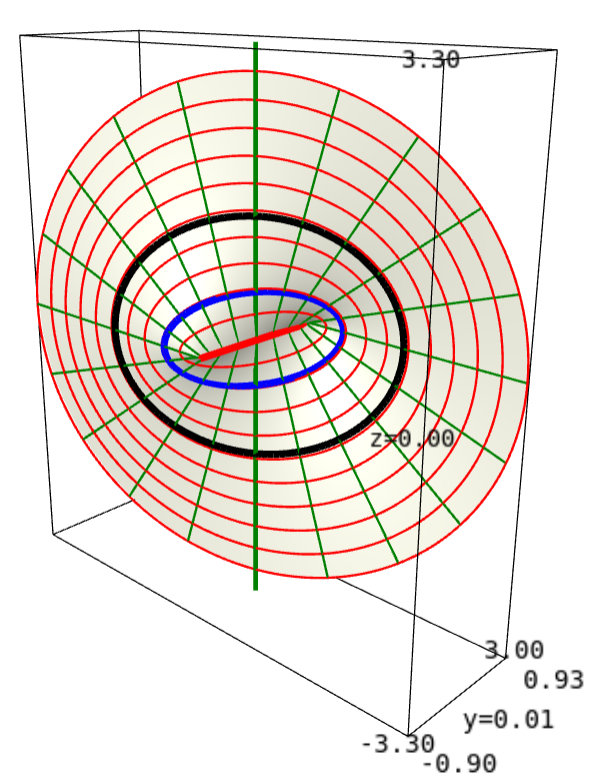
\includegraphics[width=0.45\textwidth]{ksm_phi_cut.jpg}}
\caption[]{\label{f:ksm:phi_cut} \footnotesize
Surface $\ti=\mathrm{const}$, $\tph=0$ or $\pi$ and $r\geq 0$ of the $a=0.9\, m$
Kerr spacetime depicted in terms of
the Kerr-Schild coordinates $(x,y,z)$.
The drawing is limited to $r\leq 3 m$.
The vertical thick green line is
the axis of rotation. On the right of it $\tph=0$, while on the left
of it $\tph=\pi$.
The red lines are curves $r=\mathrm{const}$,
while the green ones are curves $\th=\mathrm{const}$, which can be thought of as
the traces of the ingoing principal null geodesics.
The thick black curve marks the black hole event horizon and the thick blue curve the Cauchy horizon.
The thick red segment along the $y$-axis
marks the intersection of the surface with the disk $r=0$.
\textsl{[Figure produced with the notebook \ref{s:sam:Kerr_Schild}]}
}
\end{figure}




The identity (\ref{e:ksm:ellipsoids}) shows that, in the Euclidean space spanned by the $(x,y,z)$ coordinates,
the surfaces of constant $r\not=0$ are
confocal\footnote{In any plane containing the axis of symmetry $x^2+y^2=0$, the trace of
the ellipsoids are ellipses that share the same foci, located
at the abscissas $\pm a$ along the $z=0$ axis.}
ellipsoids of revolution.
This is depicted in Fig.~\ref{f:ksm:phi_cut}, which represents
a slice $\ti=\mathrm{const}$ and $\tph = 0$ or $\pi$ in terms of
the $(x,y,z)$ coordinates. Note that this slice is not a plane but a warped surface,
with a kink along the red segment $-a<y<a$ at $(x,z) = (0,0)$, which is the intersection
of the slice with the double disk $r=0$ (to be discussed below).
Peculiar $r=\mathrm{const}$ surfaces are
the black hole event horizon ($r=r_+=m + \sqrt{m^2 - a^2}$, cf. Sec.~\ref{s:ker:event_hor}) and the Cauchy horizon
($r = r_- = m - \sqrt{m^2 - a^2}$, cf. Sec.~\ref{s:ker:Cauchy_hor}).
They are depicted in respectively black and blue in Fig.~\ref{f:ksm:phi_cut}.

Since the ingoing principal null geodesics\index{principal!null geodesic} $\Li^{\rm in}_{(v,\th,\tph)}$
(cf. Sec.~\ref{s:ker:principal_geod}) are curves $(\th, \tph) = \mathrm{const}$,
their traces in the
3-space of Fig.~\ref{f:ksm:phi_cut} are the green lines that terminates
at the disk $r=0$ (the red segment along the $y$-axis).
Another view of the ingoing principal null geodesics is provided by
Fig.~\ref{f:ksm:theta_cut}, which shows two surfaces $(\ti,\th)=\mathrm{const}$
in terms of the Kerr-Schild coordinates $(x,y,z)$, namely the surfaces
$\th = \pi/6$ and $\th = \pi/2$. We notice that, although they are
straight lines in terms of the Kerr-Schild coordinates, the ingoing principal null geodesics are winding around the rotation axis in the direction of the black hole rotation,
which is indicated by $\w{\eta}$ [cf. Eq.~(\ref{e:ksm:eta_KS})].

\begin{figure}
\centerline{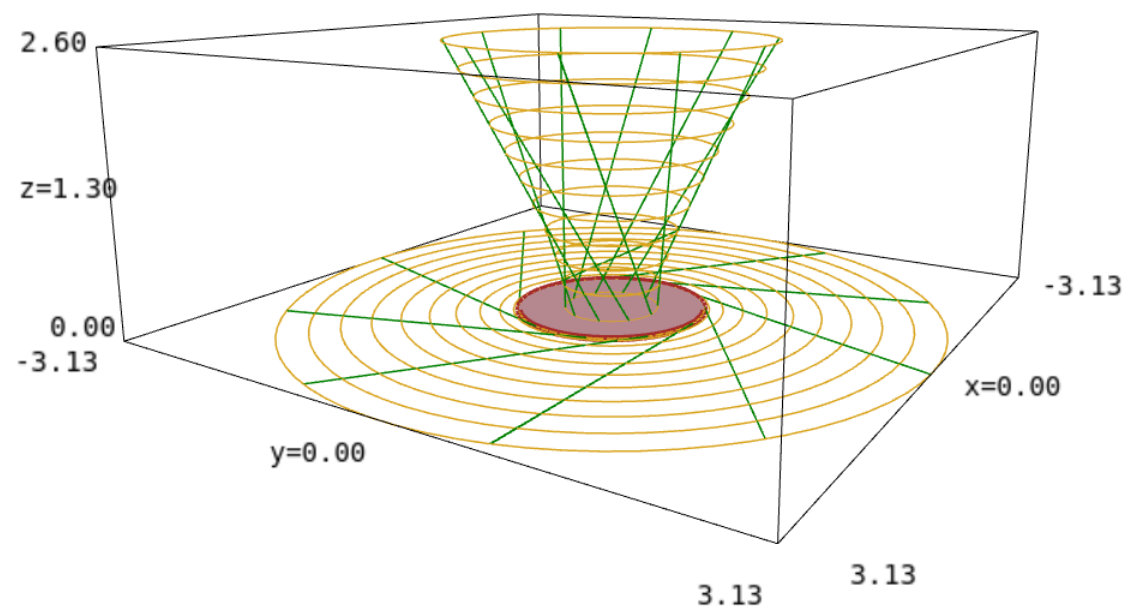
\includegraphics[width=0.7\textwidth]{ksm_theta_cut.jpg}}
\caption[]{\label{f:ksm:theta_cut} \footnotesize
Surfaces $(\ti,\th)=\mathrm{const}$ of
the $a=0.9\, m$ Kerr spacetime depicted in terms of
the Kerr-Schild coordinates $(x,y,z)$.
The disk-like surface in the plane $z=0$ is for $\th=\pi/2$, while
the cone-like surface is for $\th=\pi/6$.
The pale brown lines are curves $(r,\th)=\mathrm{const}$,
while the green ones are curves $(\th,\tph)=\mathrm{const}$. The latter
can be thought of as the traces of the ingoing principal null geodesics.
The central pink disk is the (double) disk $r=0$, the boundary of which is the
curvature singularity.
\textsl{[Figure produced with the notebook \ref{s:sam:Kerr_Schild}]}
}
\end{figure}



\subsection{The double-disk $r=0$} \label{s:ksm:r_zero}

For $r=0$, the system (\ref{e:ksm:K_to_KS}) reduces to
\begin{subequations}
\label{e:ksm:K_to_KS_r_zero}
\bea
    \ti & = & \ti \\
    x & = & - a  \sin\th \sin\tph \\
    y & = & a \sin\th \cos\tph \\
    z & = & 0
\eea
\end{subequations}
For $a\not=0$ and a fixed value of $\ti$, the subset $r=0$ of the Kerr spacetime $\M$
is the set $\mathcal{S}_{0,t}$ discussed in Sec.~\ref{s:ker:basic_prop}
[cf. Eq.~(\ref{e:ker:S_r_zero})], where $t$ is related to $\ti$ via
Eq.~(\ref{e:ker:ti_t}), which for $r=0$, is basically $\ti = t + \mathrm{const}$.
$\mathcal{S}_{0,t}$ is topologically a 2-sphere minus its equator. It is therefore
disconnected, with two connected components: the two open hemispheres,
$\mathcal{S}_{0,t}^+$ and  $\mathcal{S}_{0,t}^-$ say.
As shown in Sec.~\ref{s:ker:basic_prop}, $\mathcal{S}_{0,t}^+$ and
$\mathcal{S}_{0,t}^-$  are actually
two disks that, with respect to the metric induced by $\w{g}$, (i) have radius $a$
and (ii) are flat. The disk $\mathcal{S}_{0,t}^+$ is spanned by
the coordinates $(\th,\tph)$ with $\th\in {[0, \pi/2)}$,
while $\mathcal{S}_{0,t}^-$ is spanned by
the coordinates $(\th,\tph)$ with $\th\in {(\pi/2, \pi]}$.
Let $p\in\mathcal{S}_{0,t}^+$
be a point of Kerr coordinates $(\ti, 0, \th, \tph)$. The point
$q$ of coordinates $(\ti, 0, \pi-\th, \tph)$ belongs to
$\mathcal{S}_{0,t}^-$; it is therefore distinct from $p$, since
$\mathcal{S}_{0,t}^+$ and  $\mathcal{S}_{0,t}^-$ are two disjoint sets. Now,
the transformation (\ref{e:ksm:K_to_KS_r_zero}) maps both $p$ and $q$ to the same
value $(\ti, - a  \sin\th \sin\tph, a \sin\th\cos\ph, 0)$ of the Kerr-Schild coordinates
$(\ti, x, y, z)$. We conclude that, for $r=0$, the Kerr-Schild coordinate system fails
to establish a one-to-one correspondence between the manifold points and
some open subset of $\R^4$. Actually, as it is clear from (\ref{e:ksm:K_to_KS_r_zero}),
the two disks $\mathcal{S}_{0,t}^+$ and  $\mathcal{S}_{0,t}^-$ are mapped
by Kerr-Schild coordinates to a single disk, namely the disk of radius $a$ centered
at $(x,y,z)=(0,0,0)$ in the plane $z=0$. This disk is shown in
Fig.~\ref{f:ksm:theta_cut} (pink central disk) and in Fig.~\ref{f:ksm:rzero_disk};
its section $\tph = 0$ or $\pi$
is depicted as the red segment in Fig.~\ref{f:ksm:phi_cut}.
The disk boundary is the circle $z=0$, $\sqrt{x^2 + y^2} = a$; it is not part
of $\M$, being the curvature singularity of Kerr spacetime
(cf. Sec.~\ref{s:ker:singularities}).



\begin{figure}
\centerline{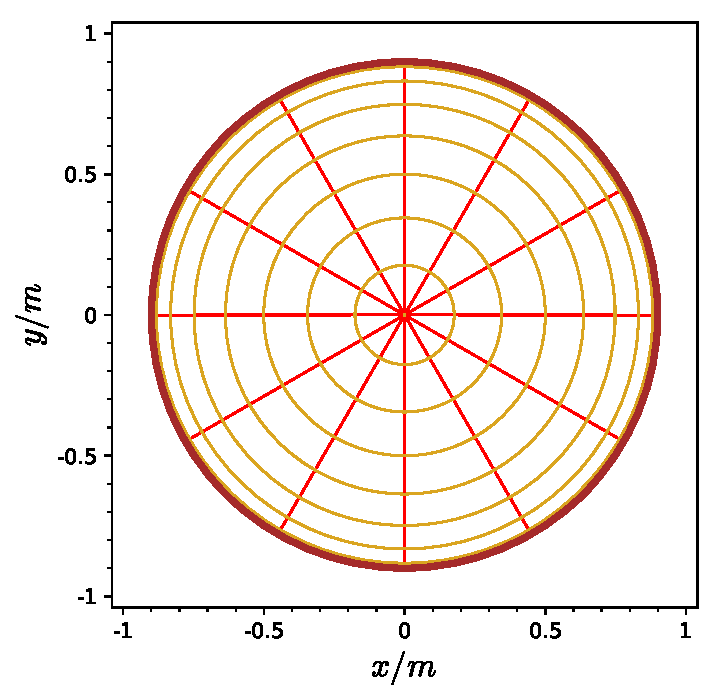
\includegraphics[width=0.45\textwidth]{ksm_rzero_disk.pdf}}
\caption[]{\label{f:ksm:rzero_disk} \footnotesize
Disk (actually double disk) $r=0$ of the $a=0.9\, m$ Kerr spacetime depicted in terms of
the Kerr-Schild coordinates $(x,y)$. The pale brown circles are the curves
$\th=\mathrm{const}$, while the red segments are the curves $\tph=\mathrm{const}$.
The disk boundary at
$\sqrt{x^2 + y^2} = a$ is the curvature singularity
of Kerr spacetime.
\textsl{[Figure produced with the notebook \ref{s:sam:Kerr_Schild}]}
}
\end{figure}

\begin{figure}
\begin{minipage}[c]{0.33\textwidth}
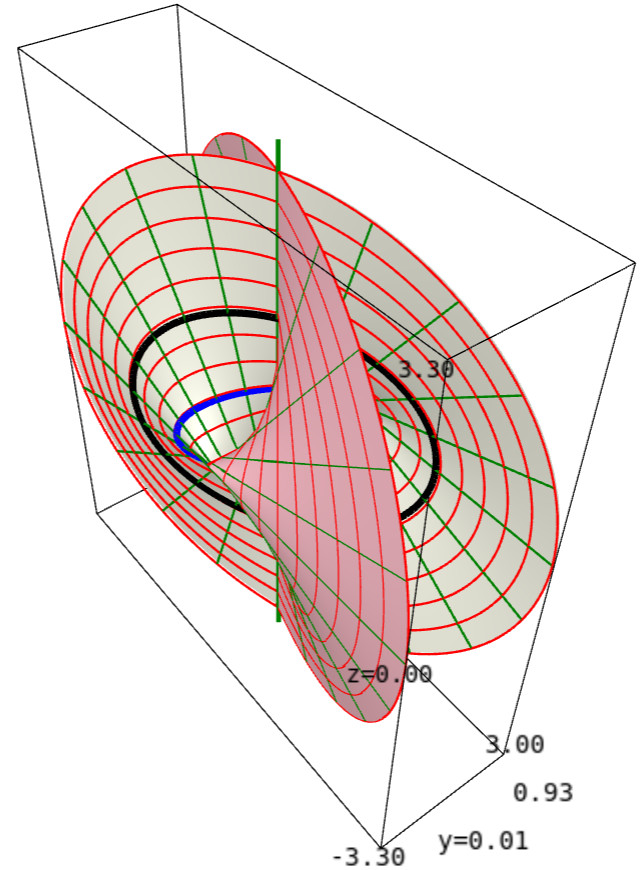
\includegraphics[height=0.35\textheight]{ksm_2_sheets.jpg}
\end{minipage}
\hfill
\begin{minipage}[c]{0.33\textwidth}
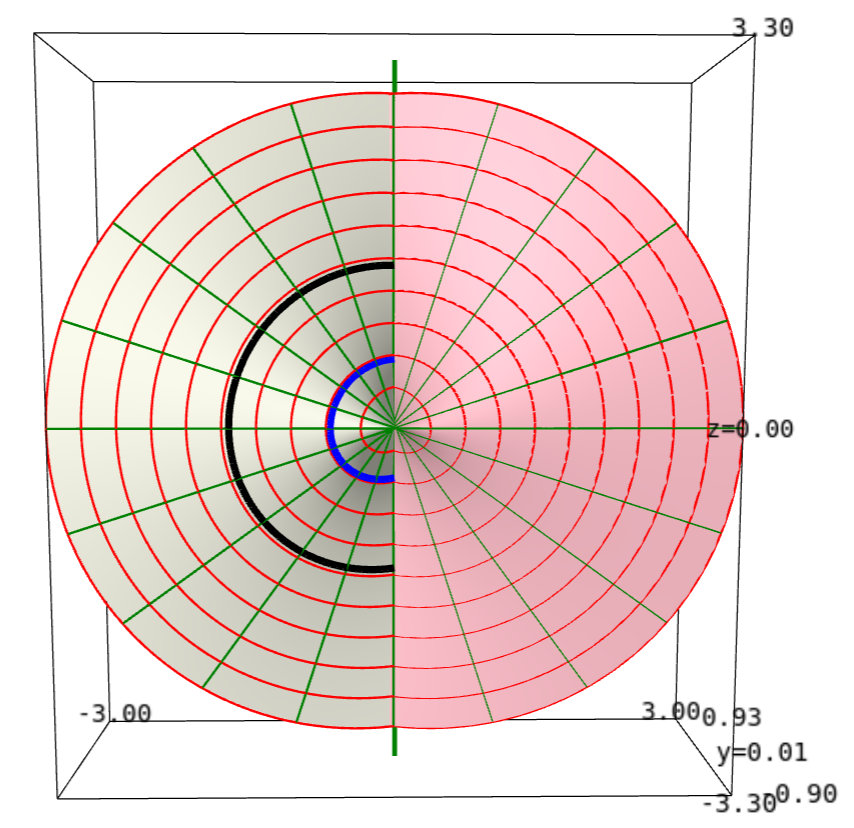
\includegraphics[height=0.25\textheight]{ksm_2_sheets_face_on.jpg}
\end{minipage}
\hfill
\begin{minipage}[c]{0.2\textwidth}
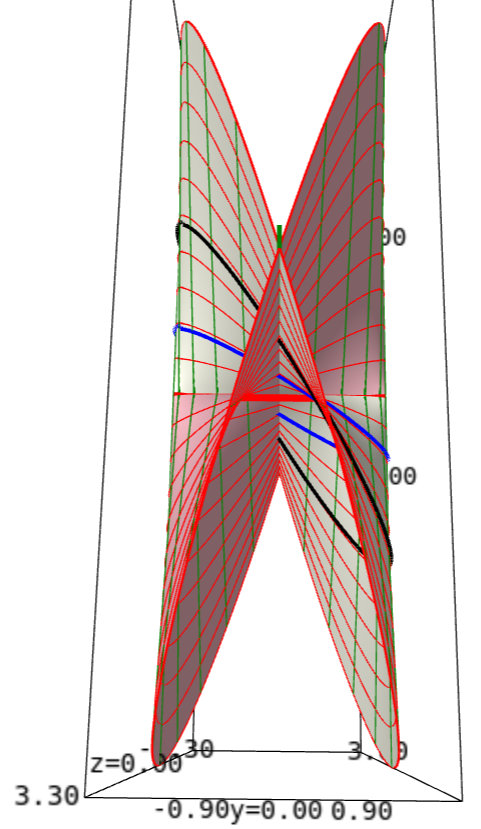
\includegraphics[height=0.3\textheight]{ksm_2_sheets_top.jpg}
\end{minipage}
\caption[]{\label{f:ksm:2_sheets} \footnotesize
Three views of the
immersion of the full $\ti=\mathrm{const}$ and $\tph=0$ or $\pi$ surface of the $a=0.9\, m$
Kerr spacetime in the Euclidean space $\mathbb{R}^3$, using the Kerr-Schild coordinates
$(x,y,z)$ for the $r\geq 0$ part (drawn in grey) and the Kerr-Schild coordinates
$(x',y',z')$ for the $r\leq 0$ part (drawn in pink). The red lines are curves
$(r,\tph)=\mathrm{const}$, while the green straight lines are ingoing principal null
geodesics, which obey $(\th,\tph) = \mathrm{const}$. The thick (resp. blue) black curve marks the black hole event horizon (resp. Cauchy horizon).
\textsl{[Figure produced with the notebook \ref{s:sam:Kerr_Schild}; see this notebook
for an interactive 3D view]}
}
\end{figure}


\subsection{Kerr-Schild coordinates on the $r\leq 0$ part}

On the domain $\M_-$, i.e. for $r\leq 0$,
one can introduce another patch of Kerr-Schild coordinates, $(\ti,x',y',z')$ say,
by formulas similar to (\ref{e:ksm:K_to_KS}). A difference is when expressing
the square root for $r$ as in Eq.~(\ref{e:ksm:r_xyz}), one has to take the
minus sign, so that
\be
    r := - \sqrt{ \frac{1}{2} \left(
        {x'}^2 + {y'}^2 + {z'}^2 - a^2 +
        \sqrt{({x'}^2 + {y'}^2 + {z'}^2 - a^2)^2 + 4 a^2 {z'}^2} \right)} .
\ee
The two Kerr-Schild coordinate domains $\M_+$ and $\M_-$ are connected through
the $r=0$ hypersurface. On a $\ti=\mathrm{const}$ slice, this means being
connected through the double disk $\mathcal{S}_{0,t}$. Such a connection
is depicted in Fig.~\ref{f:ksm:2_sheets}, which represents the (non-isometric)
immersion in $\mathbb{R}^3$ of the surface $\ti=\mathrm{const}$ and $\tph\in\{0,\pi\}$,
with $r$ ranging from $-\infty$ to $+\infty$ (actually from $-3m$ to $3m$
on the figure). The immersion is not an embedding\footnote{See Sec.~\ref{s:bas:embed}
for the definitions of \emph{immersion} and \emph{embedding}.} because the
sheet $r\geq 0$ (in grey) intersects the sheet $r\leq 0$ (in pink) along the
rotation axis, while the only intersection of $\M_+$ and $\M_-$ is along
the double disk $\mathcal{S}_{0,t}$ (reduced to the segment $-a < y< a$ at
$(x,z) = (0,0)$ in Fig.~\ref{f:ksm:2_sheets}). In other words, the intersection
of the grey and pink sheets along the $z$-axis in Fig.~\ref{f:ksm:2_sheets}
is spurious (does not correspond to an intersection in the physical spacetime),
while the intersection along the $y$-axis is physical.
From the central and right views in Fig.~\ref{f:ksm:2_sheets}, one sees clearly
that the ingoing principal null geodesics go smoothly from the $r > 0$ region
to the $r < 0$ region through $\mathcal{S}_{0,t}$.


\subsection{Link with Boyer-Lindquist coordinates}

The link between the Kerr-Schild coordinates $(\ti,x,y,z)$ and the Boyer-Lindquist
coordinates $(t,r,\th,\ph)$
is obtained by combining Eqs.~(\ref{e:ksm:K_to_KS}) with Eqs.~(\ref{e:ker:Kerr_3p1_BL_int}).


\begin{hist}
Kerr-Schild coordinates on Kerr spacetime have been introduced by Roy Kerr\index[pers]{Kerr, R.P.} in the famous 1963 paper
\cite{Kerr63} announcing the discovery of the
Kerr metric. They have been discussed further by Robert Boyer\index[pers]{Boyer, R.H.} and Richard Lindquist\index[pers]{Lindquist, R.W.}
in 1967 \cite{BoyerL67}, Brandon Carter\index[pers]{Carter, B.} in 1968
\cite{Carte68a}
and Stephen Hawking\index[pers]{Hawking, S.W.} and George Ellis\index[pers]{Ellis, G.F.R.} in 1973 \cite{HawkiE73}.
Generic Kerr-Schild metrics have been introduced and studied by Roy Kerr and Alfred
Schild\index[pers]{Schild, A.}
in 1965 \cite{KerrS65}.
\end{hist}
